
\chapter{Literature Review}



\section{Related Work}


Autonomous navigation for UAVs has been widely researched, with prominent methods like Simultaneous Localization and Mapping (SLAM) providing comprehensive mapping and localization. SLAM allows UAVs to construct detailed maps while tracking their position within it {arafat2023vision}. Typically, SLAM combines multiple sensors—such as cameras, LiDAR, and IMUs—to achieve accurate localization, making it particularly effective in indoor, repetitive environments like warehouses. However, building and maintaining a high-resolution map in SLAM is computationally intensive, consuming significant processing power and memory {arafat2023vision}. This makes it challenging for real-time applications in resource-limited UAVs. Additionally, SLAM is sensitive to map distortions and inaccuracies, which can degrade localization reliability {arafat2023vision}. Furthermore, UAV navigation generally requires only localized terrain data relevant to immediate surroundings, making SLAM excessive for UAV applications.

Optical flow is another technique used to estimate motion by tracking pixel shifts between frames, relying on the assumption of small, smooth movements \cite{odonovan2005optical}. This brightness constancy assumption fails with abrupt UAV movements, rotations, or scale changes, leading to unreliable motion estimates. Furthermore, optical flow is computationally intensive when calculating dense flow across entire frames, making it less suitable for real-time processing on resource-constrained UAVs \cite{barnum2003practical}.

Various studies specifically address UAV navigation through image-based solutions, leveraging feature matching techniques to estimate location.

The first study presents an image-based location estimation approach that combines relative positioning techniques through aerial image sequences to improve short-term odometry, enhancing UAV navigation reliability over short distances. This method emphasizes the importance of constant global correction but does not consider a solution that uses fixed reference images for navigation \cite{sim2002integrated}.

Another method, LoFTRS, uses deep learning-based image matching with semantic constraints to improve matching accuracy, providing refined feature correspondence that strengthens subsequent UAV localization tasks \cite{Zhang2024}. While this study offers valuable insights into potential pipelines, it lacks a detailed implementation and comparison of various methods across different terrains.

Ultimately, these methods do not provide a complete navigation pipeline, real-time adaptability, or testing across diverse, challenging, typical UAV conditions. Implementation details required for practical use in varied environments are also absent, limiting their proof of robustness in real-world scenarios.

This study addresses these gaps by presenting a comprehensive pipeline designed for UAVs, incorporating in-depth method comparisons, environmental adaptability, and rigorous testing under adverse conditions, making it a reliable and scalable framework for solving real-world UAV navigation challenges through image comparisons. 


% -----------------------------------------------------------------------------------------------------------------------------------

\section{Background}

This section provides a comprehensive overview of the fundamental concepts and techniques that underpin the proposed image-based UAV navigation system. By delving into feature extraction, matching, and planar transformations, it establishes the theoretical foundation essential for the subsequent system design and implementation. The discussion emphasizes the critical role of feature-based methods over direct approaches, setting the stage for understanding the chosen methodologies.


% -----------------------------------------------------------------------------------------------------------------------------------



\subsection{Feature Detectors}

Feature extraction is a cornerstone of image-based UAV navigation, enabling the estimation of transformations such as rotation and translation between consecutive images. Feature detectors identify \textbf{keypoints}—distinct, repeatable points within an image—and generate \textbf{descriptors} that encapsulate information about the local image region surrounding each keypoint. These keypoints and descriptors are essential for accurate matching across multiple frames, allowing the system to track movement while maintaining invariance to changes in scale, rotation, and illumination. This precision is critical for accurately inferring both rotational and translational shifts between images. An example of feature detection and matching, to be explained in the subsequent section, is illustrated in Figure \ref{fig:feature_detection} as outputted by the navigation system. This image shows the top 50 matches between two images after rotational alignment. 

\begin{figure}[H]
    \centering
    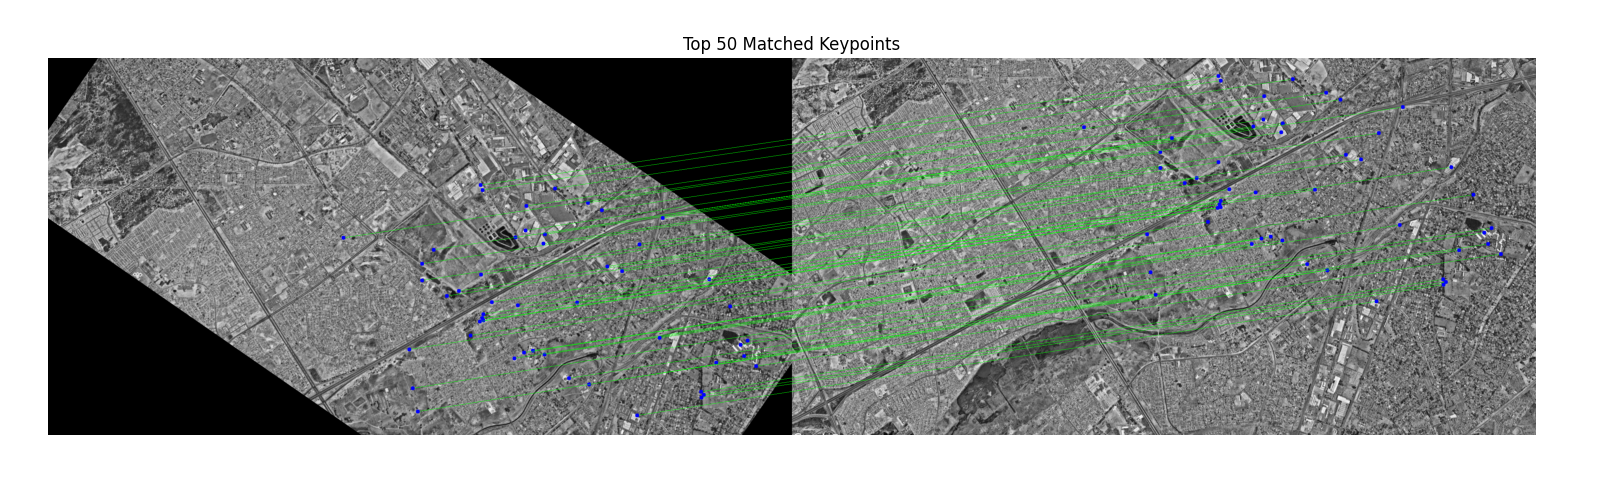
\includegraphics[width=0.94\textwidth]{./Chapter 2/litfigs/matche.png}
    \caption{Feature Detection and Matching; adapted from \cite{GoogleEarth}.}
    \label{fig:feature_detection}
\end{figure}



In this context, \textit{features} refer to both keypoints and descriptors, as each feature extraction method provides both components to facilitate effective image matching. The selection of feature extractors focuses on a subset of the most influential, efficient and accurate detectors that are free from patent restrictions.


\subsubsection{ORB (Oriented FAST and Rotated BRIEF)}

\textbf{ORB} combines the \textbf{FAST} \cite{trajkovic1998fast} keypoint detector with the \textbf{BRIEF} \cite{calonder2010brief} descriptor, enhanced for rotation invariance. \textbf{FAST} rapidly identifies keypoints by analyzing pixel intensity differences in a circular region around each candidate point. Once detected, \textbf{BRIEF} encodes the local image patch into a binary string through intensity comparisons. ORB introduces rotational invariance by aligning keypoints based on their dominant orientation before descriptor computation. This enhancement makes ORB both extremely fast and robust to scale and in-plane rotation, although it may struggle with repetitive textures or complex lighting variations \cite{tareen2018comparative}. 

\subsubsection{AKAZE (Accelerated-KAZE)}

\textbf{AKAZE} constructs a nonlinear scale space using diffusion-based filtering, capturing finer image details more effectively than linear methods. It detects keypoints by assessing local contrast with a specialized adaptive filter, enabling the identification of subtle features that simpler detectors might miss. The \textbf{Modified Local Difference Binary (MLDB)} \cite{reddy2021implementation} descriptor encodes the neighborhood of each keypoint into a binary vector based on pixel intensity differences. While AKAZE is both fast and compact, its performance can be sensitive to detection thresholds across different environments, potentially affecting its robustness in varied operational contexts \cite{opencv_akaze}. However, a notable strength of AKAZE is its its rotational invariance \cite{tareen2018comparative}. 

\subsubsection{SuperPoint with LightGlue}

\textbf{SuperPoint} is a deep learning-based keypoint detector and descriptor that leverages convolutional neural networks (CNNs) to identify and describe keypoints in a single forward pass. Pre-trained on extensive image datasets, SuperPoint excels at recognizing stable and distinctive keypoints under varied conditions \cite{rpaultrat2023superpoint}. However, its performance may degrade on datasets significantly different from its training data. Pairing SuperPoint with \textbf{LightGlue}, a machine-learning-based matcher, enhances matching accuracy through advanced graph-based techniques that were recognized at the 2023 International Conference on Computer Vision \cite{cvg2023lightglue}. Despite their high accuracy, SuperPoint and LightGlue are computationally intensive, necessitating GPU acceleration for real-time applications; however, their improved performance justifies their testing in this study, noting that they will not perform in real-time when testing with only a CPU \cite{rpaultrat2023superpoint}.

% -----------------------------------------------------------------------------------------------------------------------------------


\subsection{Feature Matching}

Feature matching establishes correspondences between keypoints in different images based on descriptor similarity. After identifying these correspondences, ambiguities and low-quality matches are removed, as detailed in Section ~\ref{sec:Optimization Techniques}. 

Each matcher generates a list of potential matches along with their similarity scores, quantified using a descriptor-space distance metric. These scores are instrumental in subsequent filtering processes.

Feature matching involves two primary components: the choice of matching technique to acquire potential matches and the search technique that determines which of these matches to retain. 

\subsubsection{Types of Feature Matching Techniques}

The following match acquisition techniques are commonly employed in feature-based navigation systems:

\textbf{Brute-Force Matcher (BFMatcher)}: The Brute-Force Matcher is a simple, exhaustive matcher that matches each feature in one image with every feature in the second image, ensuring the best possible match based on descriptor similarity. While this guarantees high accuracy, it is computationally expensive, especially with large numbers of keypoints, making it less suitable for real-time applications without optimization \cite{opencv_bfmatcher}.

\textbf{Fast Library for Approximate Nearest Neighbours (FLANN)}: FLANN accelerates the nearest neighbour search in high-dimensional descriptor spaces using algorithms such as KD-trees or hierarchical clustering, adapting dynamically to the dataset. This approximate matching approach offers significant speed improvements with minimal loss in accuracy, making it ideal for real-time applications with extensive datasets \cite{muja2014scalable}.

\textbf{LightGlue}: Leveraging deep learning, LightGlue involves both a matching and search technique, and improves matching accuracy by employing advanced graph-based techniques to establish more reliable correspondences. Although highly effective, its structure necessitates the use of other neural network-based feature extractors like SuperPoint to realize its full potential \cite{cvg2023lightglue}. The enhanced accuracy comes at the cost of increased computational demands, requiring GPU acceleration for optimal performance.

The following search techniques are commonly used to filter matches and retain only the most reliable correspondences:

\textbf{Radius Search}: This method retains matches within a specified distance in descriptor space, effectively filtering out weaker matches. However, it does not guarantee a fixed number of matches per keypoint, leading to inconsistent results \cite{opencv_matcher_tutorial}.

\textbf{K-Nearest Neighbours (KNN) Matching}: KNN matching retains the top K matches for each keypoint, allowing the application of post-filtering techniques such as Lowe’s ratio test to eliminate ambiguous matches \cite{opencv_matcher_tutorial}.

\textbf{Vanilla Matching}: Vanilla matching returns the single best match for each keypoint based on the closest descriptor distance. It is a subset of KNN matching with K=1, offering simplicity and ease of implementation \cite{opencv_matcher_tutorial}.




% ------------------------------------------------------------------------------------------------------------------------

\subsection{Image Similarity Computation}

Image similarity computation is a pivotal component of UAV navigation systems that rely on reference images for accurate localization and pose estimation. Effective similarity measures ensure efficient processing of extensive image datasets and facilitate precise transformation estimations, which are essential for reliable navigation.

\subsubsection{2.2.3.1 Proximity-Based Techniques}

To achieve efficient, real-time performance, the search space is reduced to images within the proximity of UAV's last known location, filtering images within a static or dynamic radius. While this method is highly efficient, it does not account for potential deviations from the expected flight path or the presence of poor-quality reference images. This limitation implicates that this measure cannot be used as the sole basis for image similarity computation, necessitating the integration of additional techniques for comprehensive assessment.

\subsubsection{2.2.3.2 Global Matching Techniques}

To ensure images are evaluated for similarity and ensure they are free from significant distortion, global matching, or direct methods are employed. Direct methods estimate planar transformations by comparing entire image pixel intensities and minimizing differences through optimization techniques like gradient descent. Due to their entire context, they are well-suited for similarity comparisons, but they are not ideal for precise transformation estimation due to their sensitivity to noise and illumination changes \cite{GlobalLocal2023}. The following methods are global matching techniques commonly used in image similarity computation:


\textbf{Cross-Correlation}

Cross-correlation measures similarity by sliding one image over another and computing the sum of pixel-wise multiplications at each position. The peak value signifies the best alignment, and its magnitude indicates the confidence level of the similarity. Higher confidence values reflect greater similarity between the images. While straightforward to implement, cross-correlation is sensitive to noise and illumination changes, which can compromise the reliability of the similarity measure \cite{sharma2022crosscorrelation}.

\textbf{Histograms}

Histogram comparison assesses similarity by analyzing the distribution of pixel intensities within each image. Typically, each image's histogram is divided into 256 intensity bins for 8-bit images, and similarity is quantified using metrics such as Chi-Square or Bhattacharyya distance. This method emphasizes global color and brightness distributions but neglects spatial information, making it less effective for nuanced structural differences \cite{rosebrock2014comparehistograms}.

\textbf{Structural Similarity Index (SSIM)}

SSIM evaluates similarity by decomposing images into luminance, contrast, and structure components. It computes local statistics within small windows and integrates them into a single similarity score that mirrors perceived image quality. SSIM effectively captures structural information like edges and textures, aligning closely with human visual perception. Although slightly more computationally expensive than the former methods, it is robust to varied conditions \cite{rosebrock2017imagedifference}. 


\textbf{Local Detectors Conversion}
Although not inherently a global matching technique, local feature matching can be adapted to achieve a global understanding of image similarity. This involves identifying and matching keypoints in both images and assessing the overall number of good matches. However, this approach alone does not ensure an even distribution of matches across the entire image, potentially leading to biased, localized similarity assessments. To mitigate this, a grid matching technique is employed, dividing the image into grids and limiting the number of matches per grid. Although the most computationally intensive, this method enhances robustness against distortions and rotations by ensuring a uniform distribution of matches across the image. To maintain reasonable runtime, this method has to employ a very crude detection and matching layer. 



% -----------------------------------------------------------------------------------------------------------------------------------


\subsection{Planar Transformation Estimators}

Feature-based methods extract and match keypoints from both reference and real-time images, often incorporating outlier removal stages \cite{GlobalLocal2023}. By focusing on distinctive features rather than every pixel, these methods excel in handling large viewpoint changes and rotations, enabling more precise transformation inference. This targeted approach enhances computational efficiency and robustness to environmental distortions, though it requires careful management to avoid performance degradation from variation in the number of extracted feature points. 

In typical UAV flight scenarios, the primary transformations of interest are rotation and translation, as perspective distortion, caused by 3-Dimensional structures, and shear distortion, caused when the UAV turns or generally is not parallel to the ground, are minimal at high altitudes and while the UAV is level respectively. Further, scaling is not present as per scope. The following subsections detail the primary planar transformations employed in the system.

\subsubsection{Affine Transformation}

Affine transformation captures translation, rotation, scaling, and shear, providing six degrees of freedom. It is represented by a  \(2 \times 3\) matrix that maps points from one plane to another while preserving lines and parallelism. Affine transformations are computed by estimating the affine transformation matrix between two sets of corresponding points using OpenCV's \texttt{estimateAffine2D} function \cite{opencv_warp_affine}. While versatile, the inclusion of scaling and shear introduce unnecessary error points in the UAV case. 

\subsubsection{Rigid Transformation Estimation (SVD)}

The rigid transformation via SVD preserves the shape and size of objects by estimating only rotation and translation, excluding scaling and shear. Represented by a  \(2 \times 3\) matrix, rigid transformation ensures orthogonality in the rotation component. Utilizing Singular Value Decomposition (SVD), this method minimizes the least-squares error between two point sets. The process involves: computing the weighted centroids of both point sets, centering the points by subtracting their respective centroids, calculating the covariance matrix of the centered points, performing SVD on the covariance matrix to derive the rotation matrix, and determining the translation vector based on the centroids. The resulting \(2 \times 2\) rotation matrix and \(2 \times 1\) translation vector are combined to form the rigid transformation matrix. Rigid transformation is computationally efficient and well-suited for UAV applications \cite{sorkine2017least_squares}.


\subsubsection{Partial Affine Transformation}

Partial affine transformation simplifies the full affine model by focusing solely on translation, rotation, and limited uniform scaling, offering four degrees of freedom. This transformation is also represented by a \(2 \times 3\) matrix, similar to the affine transformation but without shearing and with reduced, uniform scaling. This offers similar performance to the prior rigid method, but with minor additional error points due to scaling \cite{opencv_warp_affine}.

\subsubsection{Homography Transformation}

Homography transformation accounts for translation, rotation, scaling, shear, and perspective distortion, providing eight degrees of freedom. It is represented by a \(2 \times 3\) matrix and is estimated using OpenCV's \texttt{findHomography} function, typically with RANSAC for outlier rejection \cite{opencv_homography}. While homography offers greater flexibility in modeling complex, typically 3-Dimensional transformations, its additional degrees of freedom introduce unnecessary errors and computational overhead for UAV-based applications. 


% -----------------------------------------------------------------------------------------------------------------------------------
\subsection{Optimization Techniques}
\label{sec:Optimization Techniques}

Optimization techniques aim to refine the accuracy and reliability of the matched points used for transformation estimation by effectively filtering out erroneous matches and improving transformation accuracy. The following subsections detail the primary optimization methods employed in this system.

\subsubsection{Random Sample Consensus (RANSAC) for Planar Transformation}

RANSAC is a robust estimation technique used to estimate planar transformations by iteratively selecting random subsets of point correspondences to fit a model and identify inliers \cite{fisher2002ransac}. The process involves randomly selecting a minimal subset of point pairs, estimating the transformation model (e.g., affine or homography) based on the selected subset, determining the number of inliers that fit the estimated model within a predefined threshold, and repeating the process for a set number of iterations or until a sufficient inlier ratio is achieved. This approach is highly effective in datasets with significant outliers, focusing on finding a model that best fits the largest subset of inliers. However, due to its iterative nature and the need to sample repeatedly, RANSAC can result in increased runtime, particularly in larger datasets or when dealing with numerous outliers \cite{fisher2002ransac}.

\subsubsection{Local Maxima Extrema Density Selection (LMEDS) for Planar Transformation}

LMEDS is a keypoint selection method designed to prioritize areas of high feature density by identifying local maxima as keypoints for matching \cite{farin2005video}. This technique involves analyzing the image to identify regions with high feature density, selecting keypoints located at local maxima within these dense regions, and filtering out less significant keypoints to reduce redundancy and improve match quality. By concentrating on areas with high feature concentration, LMEDS ensures that keypoints represent the most distinctive and informative regions of the image, enhancing both accuracy and performance by reducing redundant keypoints and improving match quality, particularly in areas with high feature variability.

\subsubsection{Lowe's Ratio Test}

Lowe's ratio test is a widely used filtering technique used to eliminate ambiguous or false keypoint matches by comparing the distance of the best match to the second-best match \cite{bian2020gms}. For each keypoint match, the ratio of the distance of the best match to that of the second-best match is calculated, and the match is retained if this ratio is below a predefined threshold. A lower ratio indicates that the best match is significantly better than the alternatives, thereby increasing the likelihood of the match being correct. An example of Lowe's ratio test filtration are showed in figure ~\ref{fig:lowes1} and figure ~\ref {fig:lowes2}


\begin{figure}[H]
    \centering
    \begin{subfigure}[b]{0.37\textwidth}
        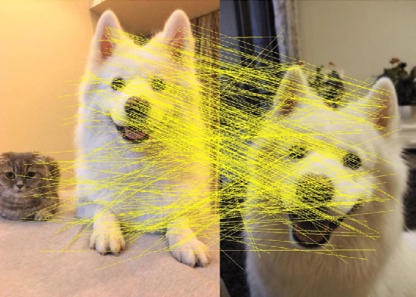
\includegraphics[width=\textwidth]{./Chapter 2/litfigs/lowes1.png}
        \caption{Matching Features Without Lowe's Ratio Test.}
        \label{fig:lowes1}
    \end{subfigure}
    \hfill
    \begin{subfigure}[b]{0.37\textwidth}
        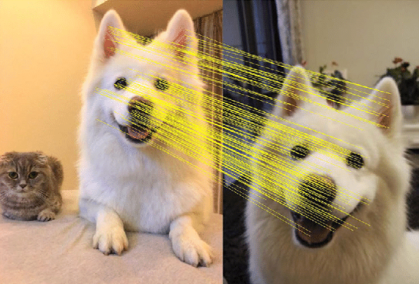
\includegraphics[width=\textwidth]{./Chapter 2/litfigs/lowes2.png}
        \caption{Matching Features With Lowe's Test.}
        \label{fig:lowes2}
    \end{subfigure}
    \caption{Reproduced from \cite{bian2020gms}.}
    \label{fig:lowes}
\end{figure}


\subsubsection{N-Match or Absolute Thresholding}
N-match thresholding involves setting a threshold that allows only a specific number of matches with the smallest descriptor distances to be retained. Absolute thresholding filters matches based on a fixed distance in descriptor space. Only matches that meet or fall below this predefined distance threshold are retained, ensuring that only sufficiently similar matches are used in the transformation estimation process. These methods primarily suffer from difficulty in setting the threshold, which is often extremely sensitive to dataset variations and method parameters.
